% --------------------------------------------------------------------------
% Template for IWAENC 2022 papers; to be used with:
%          spconfa4.sty  - ICASSP/ICIP LaTeX style file, and
%          IEEEbib.bst - IEEE bibliography style file.
%
% (Last modified by H. Loellmann, LMS, FAU Erlangen-Nuremberg, Jan. 2020)
%
% --------------------------------------------------------------------------

\documentclass{article}
\usepackage[preprint]{spconfa4}
\usepackage{amsmath,graphicx}
\usepackage[dvipsnames]{xcolor}
\usepackage{tikz}
\usetikzlibrary{arrows,snakes,backgrounds,matrix,patterns,positioning,fadings}
\usepackage{standalone}
\usepackage{subfig}
\usepackage{upgreek}
\usepackage{nicefrac}
\usepackage{dsfont}
\usepackage{bm}
\usepackage{cancel}
\usepackage{amsbsy}
\usepackage{algorithm}
\usepackage{algpseudocode}
\usepackage{lipsum}
\usepackage{harpoon}
\usepackage{comment}
\newenvironment{note}
 {\par\textcolor{Blue}{\bfseries Note:} \color{Blue}\ignorespaces}
 {\par}
\newenvironment{attention}
 {\par\textcolor{red}{\bfseries Attention:} \color{red}\ignorespaces}
 {\par}
\usepackage{hyperref}
\hypersetup{
	colorlinks,
	linkcolor={blue!80!black},
	citecolor={blue!80!black},
	urlcolor={blue!80!black}
}

\newcommand{\mtxb}[1]{\bm{\mathrm{#1}}}
\newcommand{\T}{{\mathrm{T}}}
\newcommand{\herm}{{\mathrm{H}}}
\newcommand{\ev}[1]{\mathrm{E} \left\lbrace #1 \right\rbrace}

% \excludecomment{note}
% \excludecomment{attention}

% Common variables
\newcommand{\h}{\mtxb{h}}
\newcommand{\x}{\mtxb{x}}
\newcommand{\R}{\mtxb{R}}
\newcommand{\w}{\mtxb{w}}
\newcommand{\z}{\mtxb{z}}
\newcommand{\uu}{\mtxb{u}}
\newcommand{\aRho}{\mtxb{P}}
\newcommand{\hf}{\underline{\bm{h}}}
\newcommand{\xf}{\underline{\bm{x}}}
\newcommand{\Rf}{\bm{\mathcal{R}}}
\newcommand{\wf}{\underline{\bm{w}}}
\newcommand{\zf}{\underline{\bm{z}}}
\newcommand{\uuf}{\underline{\bm{u}}}
\newcommand{\aRhof}{\bm{\mathcal{P}}}
\newcommand{\I}{\mtxb{I}}
\newcommand{\Cset}{\mathcal{C}}
\newcommand{\Csetb}{\bar{\mathcal{C}}}


% IMPORTANT: Add copyright notice by uncommenting the appropriate line
%----------------------------------------------------------
% For papers in which all authors are employed by the US government,
% \copyrightnotice{U.S. Government work not protected by U.S. copyright}

% For papers in which all authors are employed by a Crown government (UK, Canada, and Australia)
% \copyrightnotice{978-1-6654-6867-1/22/\$31.00~\copyright2022 Crown}
                   
% For papers in which all authors are employed by the European Union,
% \copyrightnotice{978-1-6654-6867-1/22/\$31.00~\copyright2022 European Union}
                   
% For all other papers the copyright notice is
\copyrightnotice{978-1-6654-6867-1/22/\$31.00~\copyright2022 IEEE}
                   
% Title.
% ------
\title{CROSS-RELATION BASED FREQUENCY-DOMAIN BLIND SYSTEM IDENTIFICATION USING ONLINE ADMM}
%
% Single address.
% ---------------
\name{Matthias Blochberger\sthanks{THANK EU!}, Filip Elvander\sthanks{THANK FWO?}, Randall Ali, Toon van Waterschoot}
\address{KU Leuven\\ESAT - Department of Electrical Engineering\\STADIUS\\3001 Leuven}
%
% For example:
% ------------
%\address{School\\
%	Department\\
%	Address}
%
% Two addresses (uncomment and modify for two-address case).
% ----------------------------------------------------------
%\twoauthors
%  {A. Author-one, B. Author-two\sthanks{Thanks to XYZ agency for funding.}}
%	{School A-B\\
%	Department A-B\\
%	Address A-B}
%  {C. Author-three, D. Author-four\sthanks{The fourth author performed the work
%	while at ...}}
%	{School C-D\\
%	Department C-D\\
%	Address C-D}
%
\begin{document}
%\ninept
%
\maketitle
%
\begin{abstract}
The abstract should appear at the top of the left-hand column of text, about 0.5 inch (12 mm) below the title area and no more than 3.125 inches (80 mm) in length.
Leave a 0.5 inch (12 mm) space between the end of the abstract and the beginning of the main text.
The abstract should contain about 100 to 150 words, and should be identical to the abstract text submitted electronically.
All manuscripts must be in English.
\end{abstract}
%
\begin{keywords}
blind system identification, multichannel signal processing, ADMM, Online-ADMM
\end{keywords}
%
\section{Introduction}
\label{sec:intro}

Its my pleasure to introduce to you: Algorithm. The most accurate, the fastest, the one most robust to noise; Simply the best you can get. Please give a warm welcome and a big applause!
\begin{attention}
    How to fit?????
\end{attention}

% \lipsum[1-4]

% #############################################################################
% #############################################################################
\section{Problem statement}
\label{sec:problem_statement}


% #############################################################################
\subsection{Signal Model}
\label{ssec:signal_model}
We define the acoustic SIMO system with the input signal \(\mtxb{s}(n) = \begin{bmatrix}
    s(n)&s(k-1)&\cdots&s(k-2L+2)
\end{bmatrix}^{\T}\) and \(i \in [M]\) outputs 
\(
    \x_i(n) = \begin{bmatrix}
        x_i(n)&x_i(k-1)&\cdots&x_i(k-L+1)
    \end{bmatrix}^{\T}
\).
Each output \(\x_i\) is the convolution of \(\mtxb{s}\) with the respective channel impulse response \(\h_i\) with additive noise term \(\mtxb{v}_i\), assumed to be zero-mean and uncorrelated.
The signal model is described by
\begin{equation}
    \x_i(n) = \mtxb{H}_i \mtxb{s}(n) + \mtxb{v}_i(n)
\end{equation}
where \(\mtxb{H}_i\) is the \(L \times (2L-1)\) linear convolution matrix of the \(i\)th channel using the elements of \(\h_i\).
\begin{note}
    Add definition of \(\mtxb{H}_i\)? Will take a lot of space.
\end{note}

% #############################################################################
\subsection{Cross-relation approach}
\label{ssec:cross_rel}
The cross-relation approach for BSI \cite{} aims to only use output signals of the system to identify it.
This is achieved by exploiting the relative channel information when more than one system output are available and certain identifiability conditions are satisfied:
\begin{itemize}
    \item Condition 1
    \item Condition 2
\end{itemize}

\noindent The fundamental equality of this approach is 
\begin{equation}
    \x_i^{\T}(n) \h_j = \x_j^{\T}(n) \h_i,\quad i,j=1,2,...,M,\,i\neq j\label{eq:cross_rel:equality_conv}
\end{equation}
which states that the output signal of one channel convolved with the impulse response of another is equal to the vice-versa.
This follows from the commutative nature of the convolution operation.
Using the (estimated) covariance \(\R_{ij} = \ev{\x_i \x_j^\T}\) instead of the signal vectors \(\x_i\) yields a more convenient problem formulation.
For the subsequent explanations the time index is dropped to make notation more compact, however the variables are time-variant.

We can combine all cross-relations \eqref{eq:cross_rel:equality_conv} into a linear system of equations
\begin{equation}
    \R \h = \bm{0} \label{eq:cross_rel:null_space}\\
\end{equation}
where 
\begin{equation}
    \R = \begin{bmatrix}
        \sum_{m \neq 1} \R_{mm} & -\R_{21} & \cdots & -\R_{M1}\\
        -\R_{12} & \sum_{m \neq 2} \R_{mm} & \cdots & -\R_{M2}\\
        \vdots & \vdots & \ddots & \vdots\\
        -\R_{1M} & -\R_{2M} & \cdots & \sum_{m \neq M} \R_{mm}\\
    \end{bmatrix},\label{eq:cross_rel:data_matrix}
\end{equation}
and \(\h = \begin{bmatrix}
    \h_1^\T & \cdots & \h_M^\T
\end{bmatrix}^\T\).
% \begin{align}
%     \R \h &= \bm{0} \label{eq:cross_rel:null_space}\\
%     \text{s.t. } \| \h \| &= a \nonumber
% \end{align}

\begin{note}
    This only has a non-zero solution when \(\R\) is not full rank i.e. has at least one eigenvalue the is zero. It is full rank though, i think. So is this formulation weird to begin with?
\end{note}

% \subsection{Frequency Domain}
% \label{ssec:frequency_domain}
This problem formulation can also be written down in the DFT domain. The derivation is analogous to the time-domain one, using the frame-based overlap-save technique \cite{}.
This gives the linear system of equations 
\begin{equation}
    \Rf \hf = \bm{0} \label{eq:frequency_domain:null_space}\\
\end{equation}
where \(\Rf\) is analogous to \eqref{eq:cross_rel:data_matrix}, however the covariance matrices replaced by the cross-spectrum matrices 
\begin{equation}
    \Rf_{ij} = \bm{\mathcal{S}}_{i}^\herm (m) \bm{\mathcal{S}}_{j}(m)
\end{equation}
with 
\begin{equation}
    \bm{\mathcal{S}}_{i} = \bm{\mathcal{W}}^{01}_{L \times 2L} \bm{\mathcal{D}}_{i}(m) \bm{\mathcal{W}}^{10}_{2L \times L}
\end{equation}
where \(\bm{\mathcal{D}}_{i}(m) = \operatorname{diag} \left\{ \operatorname{FFT}_{2L} \left\{ \x_{i,2L}(m) \right\} \right\}\) and the overlap-save matrices
\begin{align}
    \mtxb{W}_{L \times 2L}^{01} &= \begin{bmatrix}
        \mtxb{0}_{L \times L} & \mtxb{I}_{L \times L}
    \end{bmatrix}\\
    \mtxb{W}_{2L \times L}^{10} &= \begin{bmatrix}
        \mtxb{I}_{L \times L} & \mtxb{0}_{L \times L}
    \end{bmatrix}^\T\\
    \bm{\mathcal{W}}_{2L \times L}^{01} &= \mtxb{F}_{L \times L} \mtxb{W}_{L \times 2L}^{01} \mtxb{F}_{2L \times 2L}^{-1}\\
    \bm{\mathcal{W}}_{2L \times L}^{10} &= \mtxb{F}_{2L \times 2L} \mtxb{W}_{2L \times L}^{10} \mtxb{F}_{L \times L}^{-1}
\end{align} where $\mtxb{F}$ as the DFT matrix for sizes L and 2L.
The vector \(\hf\) is the stacked vector of the complex-valued spectra of the impulse responses.
In the presence of noise, the system of equations \eqref{eq:frequency_domain:null_space} is best solved by a minimization problem which seeks to minimize the squared error \(\|\underline{\bm{e}} \|^2 = \| \Rf \hf \|^2\) as
\begin{align}
    \operatorname{minimize} \quad & \hf^\herm \Rf^\herm \Rf \hf, \label{eq:frequency_domain:least_squares}\\
    \text{subject to} \quad & \hf^\herm \hf = a.
\end{align}
where the equality constraint is necessary to avoid the trivial zero solution.
As this effectively seeks for the \(a\)-scaled eigenvector corresponding to the smallest eigenvalue, we can avoid the squared matrix and replace it with its non-squared form.
To compute the estimate of the spectra, we minimize the cost function
\begin{equation}
    J(\hf) = \hf^\herm \Rf \hf\label{eq:frequency_domain:cost_function}
\end{equation}
as
\begin{align}
    \hat{\hf} = \arg \min_{\hf} \quad &\hf^\herm \Rf \hf, \label{eq:frequency_domain:min_prob}\\
    \text{s.t. } \quad &\hf^\herm \hf = a.
\end{align}
\begin{attention}
    rewrite. not nice
\end{attention}
% \begin{equation}
%     \Rf = \begin{bmatrix}
%         \sum_{m \neq 1} \Rf_{mm} & -\Rf_{21} & \cdots & -\Rf_{M1}\\
%         -\Rf_{12} & \sum_{m \neq 2} \Rf_{mm} & \cdots & -\Rf_{M2}\\
%         \vdots & \vdots & \ddots & \vdots\\
%         -\Rf_{1M} & -\Rf_{2M} & \cdots & \sum_{m \neq M} \Rf_{mm}\\
%     \end{bmatrix},\label{eq:frequency_domain:data_matrix}
% \end{equation}

% where the norm of the solution vector is constrained to some arbitrary value \(a > 0\) to avoid the trivial zero solution.

% In the presence of noise, the most convenient way to solve this problem by equating it to an error term \(\R \h = \mtxb{e}\) and minimizing this squared-error cost function
% \begin{equation}
%     J = \| \R \h \|^2 \label{eq:cross_rel:cost_function}
% \end{equation}
% which takes the form of
% \begin{align}
%     \operatorname{minimize} \quad &\| \R \h \|^2, \label{eq:cross_rel:least_squares}\\
%     \text{s.t. } \quad &\| \h \| = 1. \nonumber
% \end{align}
% The minimizer \(\hat{\h}\) of this problem is the eigenvector corresponding to the smallest eigenvalue of \(\R^\T \R\).
% This can be formulated in simpler form as
% \begin{align}
%     \hat{\h} = &\arg \min_{\h} \h^\T \R \h, \label{eq:cross_rel:min_prob}\\
%     \text{s.t. } &\| \h \| = 1, \nonumber
% \end{align}
% since the eigenvectors for the squared term \(\R^\T \R\) and the non-squared one \(\R\) are the same.
% \begin{attention}
%     Rewrite to have later section relate better. Also how to introduce Frequency domain algorithm?
% \end{attention}

% #############################################################################
% #############################################################################
\section{Review NMCFLMS(?) and friends}
\label{sec:reviewf_mc_n}
\begin{attention}
    Is there space for review? Also, does it make sense to review the time domain algorithms when this is a "frequency domain" one. 
\end{attention}
% \lipsum[5-8]

% #############################################################################
% #############################################################################
\section{Proposed Method}
\label{sec:proposed_method}
This method uses Online-ADMM to find a solution to the minimization problem posed in previous sections.
To achieve this, we introduce reduced problem with the same solution.
\begin{attention}
    Show that!
\end{attention}
This problem can be split into smaller sub-problems which can be solved in parallel to reduce computation time.

% #############################################################################
\subsection{Problem Splitting}
\label{ssec:problem_splitting}
In state-of-the-art algorithms, the minimization problem \eqref{eq:frequency_domain:min_prob} is solved in its full form.
\begin{note}
    State assumption that there as many nodes as there are channels/impulse earlier.
\end{note}
The problem is split into smaller sub-problems each defined by a subset of the full channel set \(\Cset_i \subseteq [M]\).
Following from that, we define the sets \(\Csetb_j = \left\{ i \vert j \in \Cset_i \right\}\) for \(i,j \in [M]\) representing the sub-problems a channel is part of. 
Further, \(M_i = \left| \Cset_i \right| \) and \(N_j = \left| \Csetb_j \right| \) with \(i,j \in [M]\).
\begin{attention}
    Is notation \(i \in [M]\) instead of \(i=1,...,M\) okay?
\end{attention}
We replace the cost function \eqref{eq:frequency_domain:cost_function} with the separable cost function 
\begin{equation}
    \tilde{J}(\hf) = \sum_{i=1}^M \tilde{J}_i(\wf_i)  = \sum_{i=1}^M \wf_i^\T \aRhof_i \wf_i
\end{equation}
where \(\wf_i\) is defined as the stacked vector of estimated impulse responses analogous to \(\hf\) (cf. \autoref{ssec:cross_rel}) however only using a .
Analogous, \(\aRhof\) is constructed as defined in \eqref{eq:cross_rel:data_matrix} with the reduced set of channels.
In case the channel subsets are proper \(\Cset_i \subset [M]\), this leads to sub-problems each with smaller dimensions than the original centralized problem, reducing complexity.
It does not use all cross-relations available, however this does not impact identification performance significantly. 
\begin{attention}
    Show that!
\end{attention}
In \autoref{fig:problem_splitting:problem_splitting_matrix} we try to visualize which information is used by the sub-problems compared to the centralized problem.
\begin{attention}
    Write about how and why the solution is the same (why is it actually...). The optimal solution to the smaller problems is still the stacked impulse response of the subset of channel impulse responses. Can a relation to the smallest-eigenvector comment be found?
\end{attention}


\begin{figure}
    \centering
    \includestandalone[scale=0.75]{tikz/problem_splitting_matrix}
    \caption{Problem splitting}
    \label{fig:problem_splitting:problem_splitting_matrix}
\end{figure}

% #############################################################################
\subsection{General Consensus ADMM}
\label{ssec:general_consensus_admm}
The separability of the problem can be used to take advantage of the well known alternating direction method of multipliers (ADMM).
Here more specifically, general consensus ADMM \cite{} is used 
\begin{align}
    \operatorname{minimize} \quad &\sum_{i=1}^{M} \tilde{J}_i(\wf_i)\\
    \text{subject to} \quad &(\wf_i)_j = \hf_{\mathcal{G}(i,j)},\quad i=1,...,M,\,j=1,..,M_i
\end{align}
where \(\mathcal{G}(i,j)=g\) denotes the mapping of \(L\) local variable components \((\wf_i)_j\), i.e. one of the impulse responses in the stacked vector, to the corresponding global variable components \((\hf)_g\) (cf. FIGURE). For brevity, a mapped global variable \(\tilde{\hf}_i\) with \((\tilde{\hf}_i)_j = \h_{\mathcal{G}(i,j)}\) is defined.
\begin{note}
    Better description of variables and mapping; + maybe figure to explain.
\end{note}
The real-valued augmented Lagrangian for this particular general-form consensus problem is
\begin{align}
    \mathcal{L}_{\rho} (\wf,\hf,\uuf) = \sum_{i=1}^M &\left( \wf_i^\herm \aRhof_i \wf_i + 2 \Re \left(\uuf_i^{\herm} \left(\wf_i - \tilde{\hf}_i\right)\right) \vphantom{+ \frac{\rho}{2} \left\| \wf_i - \tilde{\hf}_i \right\|^2} \right.\nonumber\\
    &\left.+ \frac{\rho}{2} \left\| \wf_i - \tilde{\hf}_i \right\|^2 \right).\label{eq:general_consensus_admm:lagrangian}
\end{align}
The ADMM then consists of the iterations
\begin{align}
    \wf_i^{k+1} &= \underset{\wf_i}{\operatorname{argmin}} \left\{ \wf_i^\T \aRhof_i \wf_i + \uuf_i^{k\,\T} \left(\wf_i - \tilde{\hf}_i^{k}\right) \vphantom{+ \frac{\rho}{2} \left\| \wf_i - \tilde{\hf}_i^{k} \right\|^2}\right.\nonumber\\
    &\left. \qquad \qquad \qquad + \frac{\rho}{2} \left\| \wf_i - \tilde{\hf}_i^{k} \right\|^2 \right\}\label{eq:general_consensus_admm:local}\\
    \hf^{k+1} &= \underset{\hf, \|\hf\| = a}{\operatorname{argmin}} \left\{ \sum_{i=1}^{M} \left( \uuf_i^{k\,\T} \tilde{\hf}_i \vphantom{\frac{\rho}{2} \| \wf_i^{k+1} - \tilde{\hf}_i \|^2} \right.\right.\nonumber\\
    &\left. \qquad \qquad \qquad \vphantom{\sum_{i=1}^{M} pp } \left.+ \frac{\rho}{2} \| \wf_i^{k+1} - \tilde{\hf}_i \|^2  \right) \right\}\label{eq:general_consensus_admm:global}\\
    \uuf_i^{k+1} &= \uuf_i^{k} + \rho \left( \wf_i^{k+1} - \tilde{\hf}_i^{k+1} \right)\label{eq:general_consensus_admm:dual}
\end{align}

\subsection{Online ADMM}
\label{ssec:online_admm}
ADMM is originally an iterative method to solve optimization problems, however under certain conditions it can be applied as an adaptive algorithm, also referred to as \emph{Online ADMM} \cite{}.
\begin{attention}
    Give conditions and why they apply here.
\end{attention}
The data term as part of \eqref{eq:general_consensus_admm:lagrangian} is time-dependent, which from here on  will be denoted with the included time index \(m\) in superscript as \(\wf_i^\T \aRhof_i^{m} \wf_i\).

The iterative form of the update steps as described in \eqref{eq:general_consensus_admm:local}-\eqref{eq:general_consensus_admm:dual} can be transformed into an adaptive one by computing a finite number at each time step \(n\) with the current data term.
In this algorithm, one ADMM iteration is applied per time step, which allows us to replace the iteration index \(k\) with the time index \(n\).

The minimization problem \eqref{eq:general_consensus_admm:local} can be solved by various methods, in this case however we perform a Newton update step of the form of
\begin{equation}
    \wf_i^{m+1} = \wf_i^{m} - \mu \bm{\mathcal{V}}_i^m \left( \aRhof_i^m \wf_i^m + \uuf_i^m + \rho\left(\wf_i^m - \tilde{\hf}_i^{m}\right)\right)\label{eq:online_admm:local_update}
\end{equation}
where \(0  <\mu\leq 1\) is a step size and \(\bm{\mathcal{V}}_i^m = \left(\aRhof_i^m + \rho \I \right)^{-1}\) is the inverse Hessian of the problem.
As this inverse is costly to compute, it is approximated by a diagonalized matrix
\begin{equation}
    \tilde{\bm{\mathcal{V}}}_i^m = \operatorname{diag} \left\{ \left( \operatorname{diag} \left\{ \aRhof_i^m \right\} + \rho \right)^{-1}\right\},
\end{equation}
similar to NMCFLMS \cite{} which is straightforward to compute.

To compute the consensus \(\hf\) we include the norm constraint \(\|\hf\| = a\) with a Lagrange multiplier \(\lambda\) in the minimization problem and replace the average of penalties with a penalty of averages as
\begin{attention}
    poetic, cite our Boy[d]
\end{attention}
\begin{align}
    \hf^{k+1} &= \underset{\hf}{\operatorname{argmin}} \left\{ \frac{\lambda}{2} \left(\hf^\T \hf - a\right)\right.\nonumber\\
    &\left. \qquad \qquad \quad + \frac{M \rho}{2} \left\| \hf - \bar{\wf}^{m+1} - \frac{1}{\rho} \bar{\uu}^{m} \right\|^2 \right\}\label{eq:online_admm:consensus_min_prob}
\end{align}
where the \(M L \times 1\) vectors \(\bar{\wf}^{m+1}, \bar{\uuf}^{m+1}\) are computed as the mapped averages
\begin{equation}
    (\bar{\wf}^{m+1})_g = \frac{1}{N_g} \sum_{\mathcal{G}(i,j)=g} (\wf_i^{m+1})_j,\quad g,i,j \in [M],
\end{equation}
and
\begin{equation}
    (\bar{\uuf}^{m})_g = \frac{1}{N_g} \sum_{\mathcal{G}(i,j)=g} (\uuf_i^{m})_j,\quad g,i,j \in [M].
\end{equation}
\begin{attention}
    UGLY AND CONFUSING??!!
\end{attention}
Setting the derivative of \eqref{eq:online_admm:consensus_min_prob} to zero and solving for the optimal Lagrange multiplier \(\lambda\), we reach the update step
\begin{equation}
    \hf^{k+1} = a\frac{\bar{\wf}^{m+1} + \frac{1}{\rho} \bar{\uuf}^{m} }{\left\| \bar{\wf}^{m+1} + \frac{1}{\rho} \bar{\uuf}^{m} \right\|}.\label{eq:online_admm:consensus_update}
\end{equation}
Algorithm \ref{alg:bsi_admm} summarizes the procedure.

\begin{algorithm}
    \caption{BSI-ADMM}\label{alg:bsi_admm}
    \begin{algorithmic}
        \For {\(n=0,1,2,...\)}
            \For{\(i \in [M]\)}
                \State Acquire new data vector \(x_i^{(t)}\)
                \State Update \(\wf_i^{(n+1)} \leftarrow \wf_i^{(n)}\)
            \EndFor
            \State Update \(\hf^{(n+1)} \leftarrow \hf^{(n)}\)
            \For{\(i \in [M]\)}
                \State Update \(\uuf_i^{(t+1)} \leftarrow \uuf_i^{(n)}\)
            \EndFor
        \EndFor
    \end{algorithmic}
\end{algorithm}

% #############################################################################
% #############################################################################
\section{Numerical Evaluation}
\label{sec:perf_eval}

First part: random impulse responses at different SNRs. Short like 64 tabs e.g.
Error measure Normalized projection misalignment
\begin{equation}
    \text{NPM}(n) = 20\,\log_{10} \left(\left\| \h(n) - \frac{\h^\T (n) \h_{\text{t}}}{\h_{\text{t}}^\T \h_{\text{t}}} \right\| \cdot \left\|\h(n)\right\|^{-1}\right)
\end{equation}
where \((\h)_i = \operatorname{IFFT} \left\{ (\hf)_i \right\}\) with \(i \in [M]\) is the estimate of the stacked IRs and \(\h_{\text{t}}\) is the true vector.
Similar to \cite{} the first experiment aims to evaluates the performance of the algorithm on randomly generated impulse responses under different SNRs.
The impulse responses of length \(L=64\) are drawn from a Normal distribution with unit variance.
The results are the median of 50 Monte-Carlo runs where the time-averaged NPM of the last \(50\) frames is taken as measurement.

\begin{figure}
    \centering
    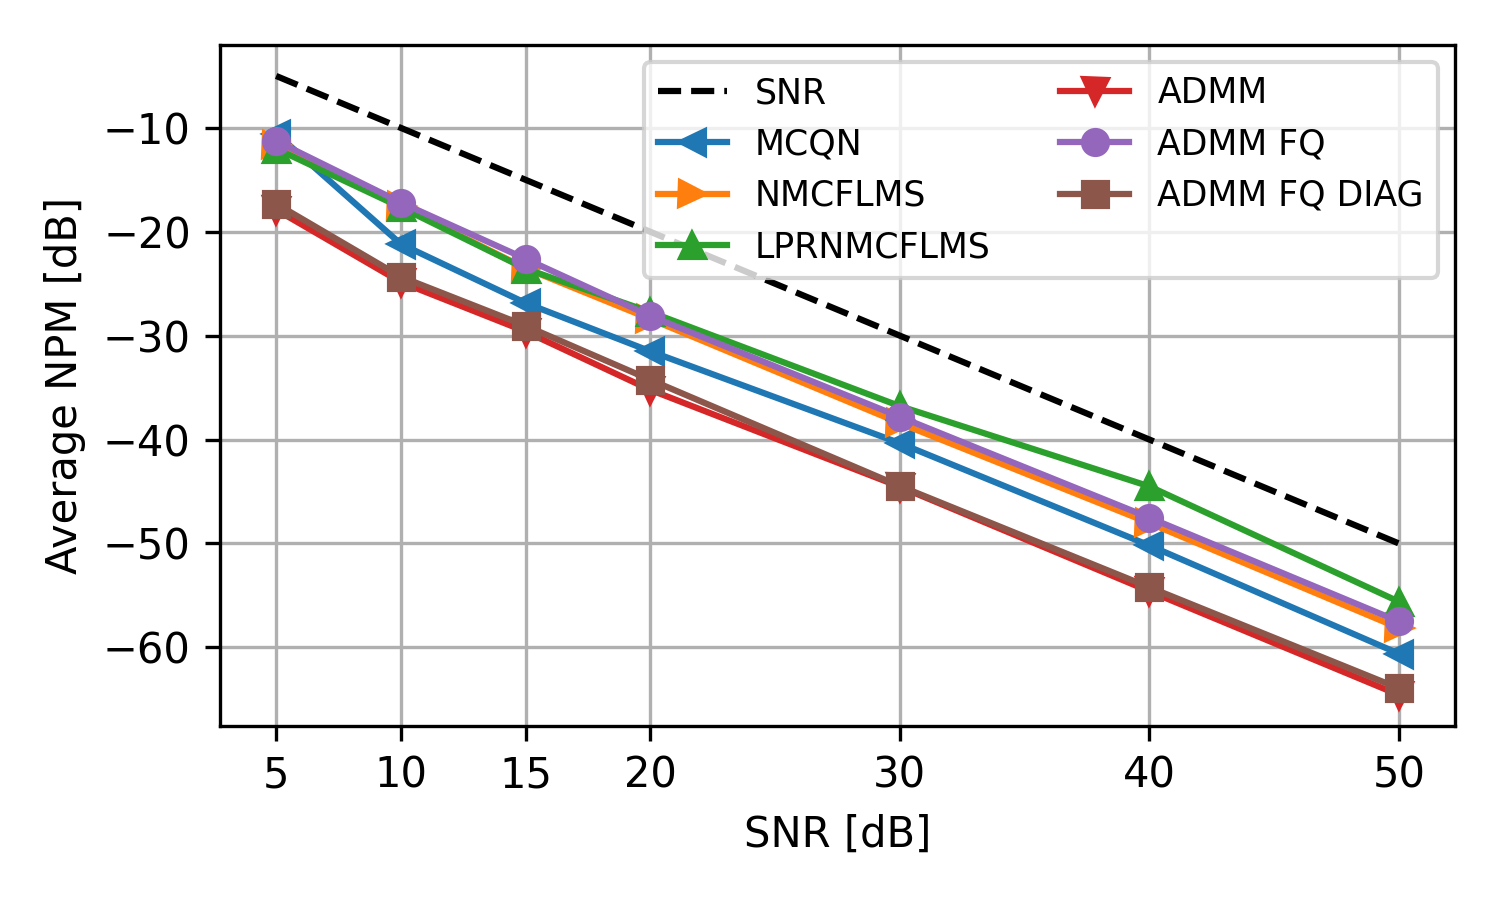
\includegraphics[width=8.5cm]{images/NPM_over_SNR.png}\label{fig:perf_eval:NPM_over_SNR}
    \caption{NPM over SNR after convergence at 8000 samples signal length. \(L=16\)}
\end{figure}


Second part: Also short IRs now evaluated over different connectivity values (less to more connections in different sized graphs)

% #############################################################################
% #############################################################################
\section{Conclusions}
\label{sec:conclusion}
LINE GO DONW

% \begin{figure}[tb]
	
% 	\begin{minipage}[b]{1.0\linewidth}
% 		\centering
% 		\centerline{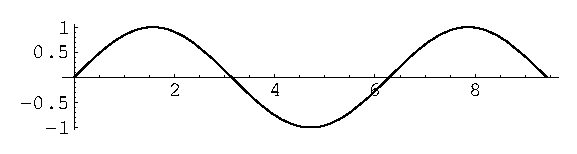
\includegraphics[width=8.5cm]{image1}}
% 		%  \vspace{2.0cm}
% 		\centerline{(a) Result 1}\medskip
% 	\end{minipage}
% 	%
% 	\begin{minipage}[b]{.48\linewidth}
% 		\centering
% 		\centerline{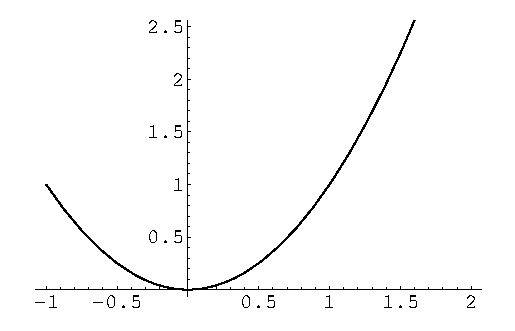
\includegraphics[width=4.0cm]{image3}}
% 		%  \vspace{1.5cm}
% 		\centerline{(b) Results 2}\medskip
% 	\end{minipage}
% 	\hfill
% 	\begin{minipage}[b]{0.48\linewidth}
% 		\centering
% 		\centerline{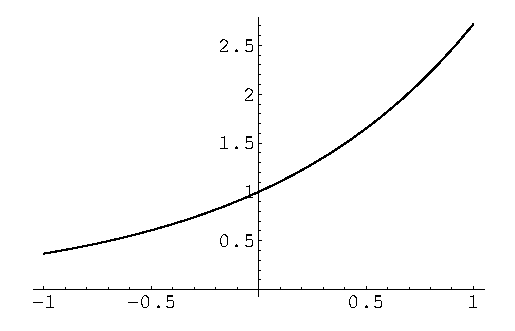
\includegraphics[width=4.0cm]{image4}}
% 		%  \vspace{1.5cm}
% 		\centerline{(c) Result 3}\medskip
% 	\end{minipage}
% 	%
% 	\caption{Example of placing a figure with results.}
% 	\label{fig:example}
% 	%
% \end{figure}

% References should be produced using the bibtex program from suitable
% BiBTeX files (here: strings, refs, manuals). The IEEEbib.bst bibliography
% style file from IEEE produces unsorted bibliography list.
% -------------------------------------------------------------------------
% \bibliographystyle{IEEEbib}
% \bibliography{refs}

\end{document}